% !TeX spellcheck = de_DE
\documentclass{uebung_cs}
\usepackage{algo223}
\uebung{2}{}{}
\blattname{Übungen zu Woche 2: Network Flow I}

%%%%%%%%%%%%%%%%%%%%%%%%%%%%%%%%%%%%%%%%%%%%%%%%%%%%%%%%%%%%%%%%%%%%%%%%%%%%
\begin{document}
\begin{exercise}[Max-Flow-Min-Cut I][\athome]
    In \cref{Figure_1,Figure_2} sind zwei Flussnetzwerke $G_1$ und $G_2$ dargestellt.
    Die Kapazität~$c(e)$ von Kante~$e$ steht dabei neben der jeweiligen Kante.
    % KT 7.1
    \begin{enumerate}
        \item Gib irgendeinen $s$-$t$-Schnitt in $G_1$ an, der \emph{nicht} minimal ist. \emph{Warum} ist dein Schnitt nicht minimal?
        \item Zähle \emph{alle} minimalen $s$-$t$-Schnitte in $G_1$ auf. Sicher, dass du alle erwischt hast?
        \item Was ist die minimale Kapazität eines $s$-$t$-Schnittes in~$G_2$? Warum?
    \end{enumerate}%
    %
    \begin{figure}[ht]
    \begin{minipage}[b]{0.5\textwidth}
        \centering
        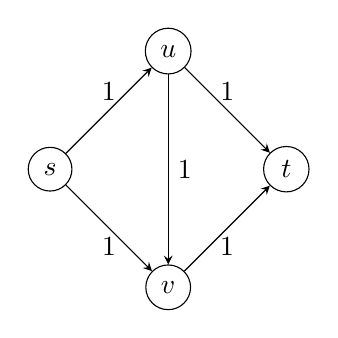
\begin{tikzpicture}
            \usetikzlibrary{arrows.meta}
            \node[draw,circle] (v0) at (1.5,3) {$u$};
            \node[draw,circle] (v1) at (0,1.5) {$s$};
            \node[draw,circle] (v2) at (3,1.5) {$t$};
            \node[draw,circle] (v3) at (1.5,0) {$v$};
            
            \path[-stealth] (v1) edge node[above] {$1$} (v0);
            \path[-stealth] (v1) edge node[below] {$1$} (v3);
            \path[-stealth] (v0) edge node[right] {$1$} (v3);
            \path[-stealth] (v0) edge node[above] {$1$} (v2);
            \path[-stealth] (v3) edge node[below] {$1$} (v2);
        \end{tikzpicture}
        \caption{\label{Figure_1}Das Flussnetzwerk~$G_1$}
    \end{minipage}
    \begin{minipage}[b]{0.5\textwidth}
        \centering
        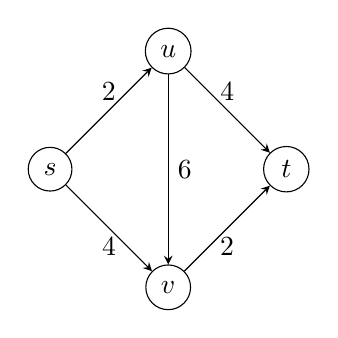
\begin{tikzpicture}
            \usetikzlibrary{arrows.meta}
            \node[draw,circle] (v0) at (1.5,3) {$u$};
            \node[draw,circle] (v1) at (0,1.5) {$s$};
            \node[draw,circle] (v2) at (3,1.5) {$t$};
            \node[draw,circle] (v3) at (1.5,0) {$v$};
            
            \path[-stealth] (v1) edge node[above] {$2$} (v0);
            \path[-stealth] (v1) edge node[below] {$4$} (v3);
            \path[-stealth] (v0) edge node[right] {$6$} (v3);
            \path[-stealth] (v0) edge node[above] {$4$} (v2);
            \path[-stealth] (v3) edge node[below] {$2$} (v2);
        \end{tikzpicture}
        \caption{\label{Figure_2}Das Flussnetzwerk~$G_2$}
    \end{minipage}
    \end{figure}
\end{exercise}

\begin{exercise}[Max-Flow-Min-Cut II][\athome]
    % KT 7.2
    \cref{Figure_3} zeigt ein Flussnetzwerk~$G_3$ sowie einen darauf definierten $s$-$t$-Fluss. Der Ausdruck $f/c$ auf jeder Kante gibt an, wie viel Fluss $f\in\N$ über die Kante geschickt wird und welche Kapazität $c\in\N$ die Kante hat.
    \begin{enumerate}
        \item Was ist der Wert des Flusses? Ist dieser Fluss ein maximaler $s$-$t$-Fluss in diesem Graphen? Warum?
        \item Finde einen minimalen $s$-$t$-Schnitt und gib dessen Kapazität an.
    \end{enumerate}
    
    \begin{figure}[ht]
	\begin{center}
		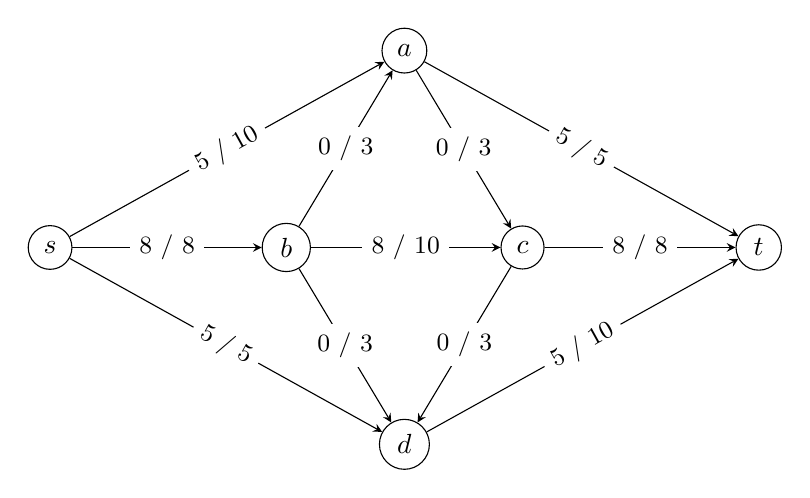
\begin{tikzpicture}
			\usetikzlibrary{arrows.meta}
			\node[draw,circle] (v0) at (4.5,  5)	    {$a$};
			\node[draw,circle] (v1) at (0,  2.5)    {$s$};
			\node[draw,circle] (v2) at (3,  2.5)	{$b$};
			\node[draw,circle] (v3) at (6,  2.5)    {$c$};
			\node[draw,circle] (v4) at (9,  2.5)	{$t$};
			\node[draw,circle] (v5) at (4.5,  0)    {$d$};
			
			\def\list {v1/v0/5/10, v1/v2/8/8, v2/v3/8/10, v3/v4/8/8, v0/v4/5/5}  % list elements
			\foreach \u\v\flow\weight in \list
			{	\draw[-stealth] (\u) -- (\v) node [fill=white, sloped, midway] {\small \flow\ $/$ \weight};
			}
			\def\vertical {v2/v0/0/3, v2/v5/0/3, v0/v3/0/3, v3/v5/0/3}  % list elements
			\foreach \u\v\flow\weight in \vertical
			{	\draw[-stealth] (\u) -- (\v) node [fill=white, midway] {\small \flow\ $/$ \weight};
			}
			\def\down {v1/v5/5/5, v5/v4/5/10} %list elements
			\foreach \u\v\flow\weight in \down
			{   \draw[-stealth] (\u) -- (\v) node [fill=white, sloped, midway] {\small \flow\ $/$ \weight};
			}
			
		\end{tikzpicture}
		\caption{\label{Figure_3}Das Flussnetzwerk~$G_3$}
	\end{center}
\end{figure}
\end{exercise}

\newpage

\begin{exercise}[Ford-Fulkerson Algorithmus][\athome]
    % Algorithms and Data Structures II - network1.pdf
    \cref{Figure_4} zeigt ein Flussnetzwerk~$G_4$.
    Führe den Ford-Fulkerson Algorithmus Schritt für Schritt aus, und berechne dadurch einen maximalen $s$-$t$-Fluss und einen minimalen $s$-$t$-Schnitt auf~$G_4$.
    
    \begin{figure}[ht]
	\begin{center}
		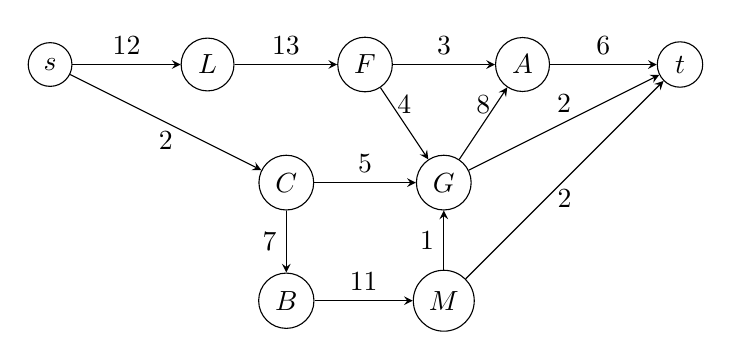
\begin{tikzpicture}
			\usetikzlibrary{arrows.meta}
			\node[draw,circle] (v0) at (0,  3.5)	{$s$};
			\node[draw,circle] (v1) at (2,  3.5)    {$L$};
			\node[draw,circle] (v2) at (4,  3.5)	{$F$};
			\node[draw,circle] (v3) at (6,  3.5)    {$A$};
			\node[draw,circle] (v4) at (8,  3.5)	{$t$};
			\node[draw,circle] (v5) at (3,    2)    {$C$};
			\node[draw,circle] (v6) at (5,    2)    {$G$};
			\node[draw,circle] (v7) at (3,  0.5)    {$B$};
			\node[draw,circle] (v8) at (5,  0.5)    {$M$};
			
			\def\list {v0/v1/12, v1/v2/13, v2/v3/3, v3/v4/6, v2/v6/4, v5/v6/5, v6/v3/8,
			v6/v4/2, v7/v8/11}  % list elements
			\foreach \u\v\weight in \list
			{	\draw[-stealth] (\u) -- (\v) node [midway, above] {\weight};
			}
			\def\vertical {v5/v7/7, v8/v6/1 %v0/v4/3, v2/v5/4, v2/v9/4%, v3/v7/7, v6/v10/1, v11/v7/2
            }  % list elements
			\foreach \u\v\weight in \vertical
			{	\draw[-stealth] (\u) -- (\v) node [midway, left] {\weight};
			}
			\def\down {v0/v5/2, v8/v4/2} %list elements
			\foreach \u\v\weight in \down
			{   \draw[-stealth] (\u) -- (\v) node [midway, below] {\weight};
			}
		\end{tikzpicture}
		\caption{\label{Figure_4}Das Flussnetzwerk~$G_4$}
	\end{center}
\end{figure}
\end{exercise}

\begin{exercise}[Eigenschaften maximaler Flüsse][\athome]\
    % KT 7.4
    Entscheide, ob die folgende Aussage wahr oder falsch ist. Wenn sie wahr ist, erkläre, warum sie das ist. Wenn sie falsch ist, gebe ein Gegenbeispiel an.
    \begin{quote}
        Sei $G$ ein beliebiges Flussnetzwerk mit einer Quelle $s$, einer Senke $t$ und einer positiven, ganzzahligen Kapazität $c_e$ auf jeder Kante $e$. Wenn $f$ ein maximaler $s$-$t$-Fluss in $G$ ist, dann saturiert $f$ jede von $s$ ausgehende Kante mit einem Fluss (d.h., für alle Kanten~$e$, die von $s$ ausgehen, gilt $f(e) = c_e$).
    \end{quote}
    (\emph{Tipp: \reflectbox{Prüfe die Aussage zunächst für kleine Beispiele, wie etwa $G_1$, $G_2$, $G_3$ und $G_4$}})
\end{exercise}

\begin{exercise}[Eigenschaften minimaler Schnitte][\atschool\mittel]\
    % KT 7.5
    Entscheide, ob die folgende Aussage wahr oder falsch ist. Wenn sie wahr ist, erkläre, warum sie das ist. Wenn sie falsch ist, gebe ein Gegenbeispiel an.
    \begin{quote}
        Sei $G$ ein beliebiges Flussnetzwerk mit einer Quelle $s$, einer Senke $t$ und einer positiven, ganzzahligen Kapazität $c_e$ auf jeder Kante $e$. Sei $(A,B)$ ein minimaler $s$-$t$-Schnitt bezüglich der Kapazitäten $\{c_e : e \in E\}$. Wenn wir jede Kapazität um~$1$ erhöhen, dann ist $(A,B)$ immer noch ein minimaler $s$-$t$-Schnitt bezüglich der neuen Kapazitäten $\{1 + c_e : e \in E\}$.
    \end{quote}
\end{exercise}

\begin{exercise}[Zombie-Ausbruch][\atschool\mittel]
    % Algorithms and Data Structures II - network1.pdf
    Im Land 1D hat ein Zombie-Ausbruch stattgefunden. Der Premierminister des Landes bittet dich, eine Lösung zu finden, um diesen Ausbruch zu stoppen. Du erhältst eine Karte des ganzen Landes, auf der die Koordinaten aller Städte verzeichnet sind. Es gibt $X$ infizierte und $Y$ noch nicht infizierte Städte. Die Karte enthält ebenso Informationen über Straßen, die die Städte miteinander verbinden. Alle Straßen sind Einbahnstraßen, das heißt sie führen in genau eine Richtung. Jede Straße führt direkt von einer Stadt in eine andere. Es gibt insgesamt $R$ Straßen. Sowohl Zombies als auch Menschen haben die Straßenverkehrsordnung so sehr verinnerlicht, dass sie sich nur auf Straßen bewegen können und auch nur in der vorgesehenen Richtung.
 
    Eine Stadt $a$ ist von einer Stadt $b$ aus erreichbar, wenn man von $b$ aus einer oder mehreren Straßen folgen kann, um nach $a$ zu gelangen. Du kannst annehmen, dass die Reise von einer Stadt in eine andere erreichbare Stadt nicht länger dauert als einen Tag.
    \begin{enumerate}
        \item \textbf{Rette die Hauptstadt!} Die Hauptstadt ist noch nicht infiziert und der Premierminister möchte wissen, wie viele Straßen zerstört werden müssen, damit die Hauptstadt verschont bleibt. Gebe einen Algorithmus an, der die minimale Anzahl an Straßen ausgibt, die zerstört werden müssen, um die Hauptstadt von den infizierten Städten abzugrenzen. Analysiere die Laufzeit deines Algorithmus in Abhängigkeit von $X$, $Y$ und $R$. Zeige, dass dein Algorithmus funktioniert.
        \item \textbf{Verteile den Impfstoff!} Wissenschaftler aus der Hauptstadt haben einen wirksamen Impfstoff gefunden. Um diesen in den noch nicht infizierten Städten zu verteilen, müssen in jede noch nicht infizierte Stadt 10 Ärzte geschickt werden. Die Ärzte können nur auf den Straßen reisen. Sie können sogar durch infizierte Städte reisen, allerdings können das nur maximal 50 Ärzte pro Stadt und Tag tun. Gebe einen Algorithmus an, der entscheidet, ob man den Impfstoff innerhalb eines Tages zu allen noch nicht infizierten Städten transportieren kann. Analysiere die Laufzeit des Algorithmus in Abhängigkeit von $X$, $Y$ und $R$. Zeige, dass dein Algorithmus funktioniert.
    \end{enumerate}
\end{exercise}

\begin{exercise}[Eine andere Sicht auf Schnitte][\atschool\note]
    Schnitte werden manchmal als Teilmengen der Kanten eines Graphen definiert anstatt als Partitionen der Knotenmenge.
    In dieser Aufgabe soll gezeigt werden, dass beide Definitionen \emph{nahezu} äquivalent sind.
  
    Sei $G$ ein gerichteter Graph mit zwei ausgezeichneten Knoten $s$ und $t$. Wir sagen, dass eine Menge $X$ von Kanten die Knoten $s$ und $t$ \emph{separiert}, falls jeder gerichtete $s$-$t$-Pfad mindestens eine Kante aus $X$ enthält.
    Für eine Menge $S$ von Knoten definieren wir
    \[\partial S \coloneqq \{u \to v : u \in S, v \not\in S\}.\]
    Somit ist $\partial S$ die Menge der gerichteten Kanten, die aus $S$ raus führen.
  
    \begin{enumerate}
      \item Sei $(S,T)$ ein beliebiger $s$-$t$-Schnitt in $G$. Beweise, dass die Kantenmenge $\partial S$ die beiden Knoten $s$ und $t$ separiert.
      \item Sei $X$ eine beliebige Teilmenge von Kanten, sodass $X$ die Knoten $s$ und $t$ separiert.
      Beweise, dass es einen $s$-$t$-Schnitt $(S,T)$ gibt, für den $\partial S \subseteq X$ gilt.
      \item Sei $X$ eine minimale Teilmenge von Kanten, sodass $X$ die Knoten $s$ und $t$ separiert.
      Beweise, dass es einen $s$-$t$-Schnitt $(S,T)$ gibt, für den $\partial S = X$ gilt.
    \end{enumerate}
  \end{exercise}
  
\begin{exercise}[Puzzle der Woche: Vier Münzen][\spass]
    % Algorithms and Data Structures II - network1.pdf
    Du musst ein Spiel gegen den Henker gewinnen. Bevor das Spiel startet, werden deine Augen verbunden. Es werden vier Münzen auf einem quadratischen Tisch platziert, sodass in jeder Ecke eine Münze liegt. Ob und welche der Münzen mit der Zahl-Seite nach oben liegen wird durch den Henker bestimmt: beliebig und für dich unbekannt. Dein Ziel ist es, dass alle vier Münzen mit der Kopf-Seite nach oben gerichtet auf dem Tisch liegen.
    
    In jeder Runde kannst du irgendeine Teilmenge von Münzen auswählen, die dann vom Henker gleichzeitig umgedreht werden. Ist danach auf allen vier Münzen der Kopf zu sehen, hast du gewonnen. Andernfalls darf der Henker den Tisch um 90, 180, 270 oder 360 Grad drehen; da deine Augen verbunden sind, weißt du nicht, welche Drehung gewählt wurde. Wenn du es nicht schaffst, in höchstens 20 Runden zu gewinnen, dann verlierst du und der Henker geht seiner eigentlichen Berufung nach. Was ist deine Strategie?
\end{exercise}

\paragraph*{Projektideen.}
Such dir im Tutorium wieder eine Gruppe und ein \emph{Projekt} aus, bei dem für dich das Feedback deines Tutors nützlich wäre.
Das kann die schriftliche Ausarbeitung einer Übungsaufgabe sein (siehe erstes Übungsblatt für die formalen Anforderungen). Oder auch diese Aufgabe:

\begin{exercise}[Implementierung von Ford-Fulkerson][\projekt\mittel]
    % Algorithms and Data Structures II - network1.pdf
    Implementiere ein Programm, das als Eingabe ein Flussnetzwerk erhält und welches mithilfe des Ford-Fulkerson Algorithmus einen maximalen Fluss zwischen zwei Knoten des Netzwerkes berechnet.
    Teste dein Programm in Coderunner (siehe {Moodle}).
\end{exercise}

\end{document}
